% tikz_colorspaces

\begin{tikzpicture} 
	
	\node[inner sep = 0pt] (n1) {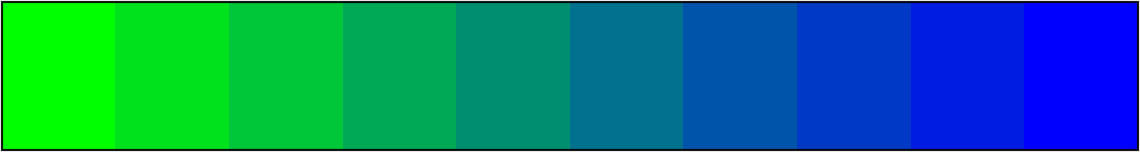
\includegraphics[width = 7cm]{\here/colorbarRGB.png}};
	\node[inner sep = 0pt, anchor = north, yshift = -0.2cm] (n2) at (n1.south)  {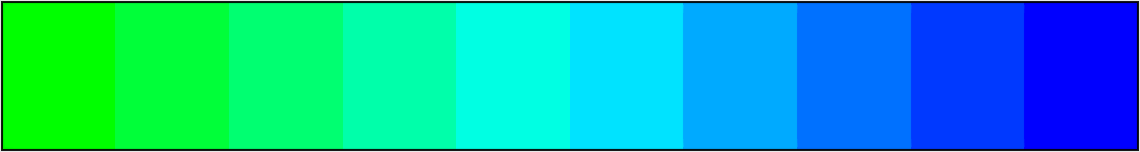
\includegraphics[width = 7cm]{\here/colorbarHSV.png}};
	\node[inner sep = 0pt, anchor = north, yshift = -0.2cm] (n3) at (n2.south) {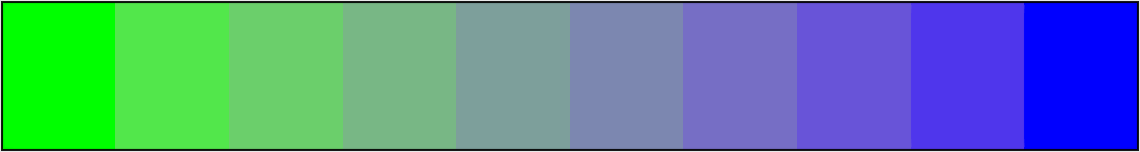
\includegraphics[width = 7cm]{\here/colorbarLab.png}};

	\node[anchor = east] at (n1.west){RGB};
	\node[anchor = east] at (n2.west){HSV};
	\node[anchor = east] at (n3.west){Lab};

\end{tikzpicture}